\documentclass{article}

\usepackage{arxiv}

\usepackage{chngcntr} % to change counter style, e.g., in appendix 

\usepackage[utf8]{inputenc} % allow utf-8 input
\usepackage[T1]{fontenc}    % use 8-bit T1 fonts
\usepackage{hyperref}       % hyperlinks
\usepackage{url}            % simple URL typesetting
\usepackage{booktabs}       % professional-quality tables
\usepackage{amsfonts}       % blackboard math symbols
\usepackage{nicefrac}       % compact symbols for 1/2, etc.
\usepackage{microtype}      % microtypography
\usepackage{lipsum}

\usepackage{float}
\usepackage{amsmath,amssymb,amsfonts}
\usepackage{algorithmic}
\usepackage[ruled, lined]{algorithm2e} % for algorithm 
\usepackage{graphicx}
\usepackage{textcomp}
\usepackage{xcolor}

%%% table
% \PassOptionsToPackage{linktocpage}{hyperref}
\usepackage{array}
\usepackage{multirow}
\usepackage{colortbl}
\usepackage{placeins}
\usepackage{float}
\usepackage{tabulary}
\usepackage[newcommands]{ragged2e}
\usepackage{lscape}
\usepackage{rotating}
\usepackage{makecell}
\usepackage[usestackEOL]{stackengine}
\usepackage{longtable}
% \usepackage{chngcntr}
% \counterwithin{table}{subsection}
\usepackage{graphicx}
\graphicspath{ {./figures/} }
\usepackage{subcaption}

\usepackage{amssymb}% http://ctan.org/pkg/amssymb
\usepackage{pifont}% http://ctan.org/pkg/pifont
\newcommand{\cmark}{\ding{51}}%
\newcommand{\xmark}{\ding{55}}%


%%% customized commands
\newcommand{\STATS}{$STATS$}
\newcommand{\SAMPnum}{$SAMP$-$NUM$}
\newcommand{\SAMPsize}{$SAMP$-$SIZE$}
\newcommand{\IAT}{$IAT$}
\newcommand{\SIZE}{$SIZE$}
\newcommand{\IATSIZE}{$IAT$+$SIZE$}
\newcommand{\IATFFT}{$IAT$-$FFT$}
\newcommand{\SIZEFFT}{$SIZE$-$FFT$}
\newcommand{\SAMPnumFFT}{$SAMP$-$NUM$-$FFT$}

\newcommand{\pkts}{PacketsSeries}
\newcommand{\bytes}{BytesSeries}

\renewcommand{\arraystretch}{1.4}   % for the vertical padding
\setlength{\tabcolsep}{15pt}
\aboverulesep=0.0ex
\belowrulesep=0.0ex
\setlength{\tabcolsep}{0.5em} % for the horizontal padding
\newcommand{\Cell}[1]{\begin{tabular}{@{}c}{\Centerstack[c]{#1}}\end{tabular}}

%# change column color
% \usepackage{xcolor,colortbl}
% \definecolor{Gray}{gray}{0.85}
% \newcolumntype{STATS}{>{\columncolor{Gray}}c}
% % \newcolumntype{STATS}{>{\columncolor{lightgray}}c}

\usepackage{changepage}                 % adjust margins for selected portions
\usepackage{lipsum}
% wide page for side by side figures, tables, etc
\newlength{\offsetpage}
\setlength{\offsetpage}{1.0cm}
\newenvironment{widepage}{\begin{adjustwidth}{-\offsetpage}{-\offsetpage}%
    \addtolength{\textwidth}{2\offsetpage}}%
{\end{adjustwidth}}

\title{xxx}


\begin{document}
\maketitle

% \begin{small}
% \scalebox{0.7}{
% \begin{table}
% \centering
\begin{longtable}[c]{|c|c|c|c|c|c|c|c|}
% \begin{tabulary}{\textwidth}{||C|C|C|C|C|C|C|C|}
% \begin{tabulary}{c|c|c||c|c|c|c|}
% \begin{tabular}{|p{2cm}|p{2cm}|p{2cm}|p{2cm}|p{2cm}|p{2cm}|p{2cm}|p{2cm}|} 
% \caption{Baseline}
\toprule
%  Detector & Dataset & STATS & SIZE & IAT & IAT+SIZE & SAMP-NUM & SAMP-SIZE  \\ 
  Detector & Dataset & STATS & SIZE & \Cell{IAT} & \Cell{IAT+\\SIZE} & \Cell{SAMP-\\NUM} & \Cell{SAMP-\\SIZE}  \\ 
\midrule
\multirow{7}{*}{OCSVM} &UNB(PC1) & 0.56 & 0.70 & 0.78 & 0.92 & 0.74 & 0.76  \\ 
&UNB(PC2) & 0.64 & 0.75 & 0.82 & 0.81 & 0.82 & 0.85  \\ 
&UNB(PC3) & 0.59 & 0.85 & 0.87 & 0.88 & 0.83 & 0.85 \\ 
&UNB(PC4) & 0.48 & 0.66 & 0.82 & 0.80 & 0.81 & 0.79 \\ 
&UNB(PC5) & 0.47 & 0.73 & 0.84 & 0.86 & 0.76 & 0.81 \\ 
\cmidrule{2-8}
&CTU & 0.98 & 0.97 & 0.95 & 0.96 & 0.88 & 0.88\\ 
\cmidrule{2-8}
&MAWI & 0.88 & 0.71 & 0.58 & 0.43 & 0.60 & 0.61\\ 
\cmidrule{2-8}
&TV\&PC & 1.00 & 1.00 & 0.96 & 0.99 & 0.95 & 0.93\\ 
\cmidrule{2-8}
&GHom & 0.76 & 0.97 & 0.70 & 0.70 & 0.95 & 0.96\\ 
&SCam & 0.58 & 0.61 & 0.56 & 0.62 & 0.56 & 0.61\\ 
&SFrig & 0.98 & 0.93 & 0.81 & 0.85 & 0.96 & 0.95 \\ 
&BSTch & 0.97 & 0.99 & 0.97 & 0.99 & 0.96 & 0.95  \\ 
\midrule
\multirow{7}{*}{IF} &UNB(PC1) & 0.49 & 0.49 & 0.51 & 0.74 & 0.66 & 0.70  \\ 
&UNB(PC2) & 0.68 & 0.61 & 0.68 & 0.75 & 0.81 & 0.80  \\ 
&UNB(PC3) & 0.62 & 0.63 & 0.70 & 0.79 & 0.81 & 0.80 \\ 
&UNB(PC4) & 0.49 & 0.51 & 0.62 & 0.65 & 0.81 & 0.79 \\ 
&UNB(PC5) & 0.55 & 0.61 & 0.69 & 0.74 & 0.79 & 0.74 \\ 
\cmidrule{2-8}
&CTU & 0.94 & 0.93 & 0.81 & 0.88 & 0.83 & 0.85\\ 
\cmidrule{2-8}
&MAWI & 0.86 & 0.70 & 0.54 & 0.67 & 0.56 & 0.55\\ 
\cmidrule{2-8}
&TV\&PC & 0.95 & 0.98 & 0.90 & 0.99 & 0.74 & 0.79\\ 
\cmidrule{2-8}
&GHom & 0.88 & 0.77 & 0.44 & 0.54 & 0.96 & 0.96\\ 
&SCam & 0.52 & 0.51 & 0.53 & 0.54 & 0.60 & 0.56\\ 
&SFrig & 0.96 & 0.96 & 0.56 & 0.94 & 0.93 & 0.93 \\ 
&BSTch & 0.97 & 0.98 & 0.94 & 0.98 & 0.98 & 0.96  \\ 
\midrule
\multirow{7}{*}{AE} &UNB(PC1) & 0.72 & 0.40 & 0.50 & 0.93 & 0.81 & 0.77  \\ 
&UNB(PC2) & 0.78 & 0.66 & 0.71 & 0.83 & 0.83 & 0.77  \\ 
&UNB(PC3) & 0.76 & 0.58 & 0.71 & 0.90 & 0.85 & 0.80 \\ 
&UNB(PC4) & 0.70 & 0.52 & 0.64 & 0.84 & 0.83 & 0.86 \\ 
&UNB(PC5) & 0.82 & 0.66 & 0.73 & 0.87 & 0.88 & 0.87 \\ 
\cmidrule{2-8}
&CTU & 0.91 & 0.96 & 0.85 & 0.96 & 0.83 & 0.87\\ 
\cmidrule{2-8}
&MAWI & 0.56 & 0.58 & 0.50 & 0.70 & 0.58 & 0.55\\ 
\cmidrule{2-8}
&TV\&PC & 1.00 & 1.00 & 0.97 & 0.99 & 0.85 & 0.95\\ 
\cmidrule{2-8}
&GHom & 0.84 & 0.69 & 0.35 & 0.86 & 0.97 & 0.96\\ 
&SCam & 0.63 & 0.61 & 0.57 & 0.65 & 0.61 & 0.60\\ 
&SFrig & 0.95 & 0.85 & 0.72 & 0.92 & 0.96 & 0.96 \\ 
&BSTch & 0.97 & 0.93 & 0.98 & 0.99 & 0.96 & 0.96  \\ 
\midrule
\multirow{7}{*}{KDE} &UNB(PC1) & 0.34 & 0.58 & 0.68 & 0.92 & 0.74 & 0.76  \\ 
&UNB(PC2) & 0.61 & 0.73 & 0.82 & 0.80 & 0.81 & 0.80  \\ 
&UNB(PC3) & 0.53 & 0.84 & 0.84 & 0.87 & 0.82 & 0.85 \\ 
&UNB(PC4) & 0.47 & 0.63 & 0.76 & 0.80 & 0.81 & 0.85 \\ 
&UNB(PC5) & 0.53 & 0.69 & 0.84 & 0.86 & 0.75 & 0.82 \\ 
\cmidrule{2-8}
&CTU & 0.96 & 0.93 & 0.94 & 0.97 & 0.82 & 0.84\\ 
\cmidrule{2-8}
&MAWI & 0.88 & 0.48 & 0.57 & 0.43 & 0.60 & 0.57\\ 
\cmidrule{2-8}
&TV\&PC & 1.00 & 1.00 & 0.96 & 0.99 & 0.88 & 0.93\\ 
\cmidrule{2-8}
&GHom & 0.60 & 0.97 & 0.71 & 0.72 & 0.96 & 0.96\\ 
&SCam & 0.52 & 0.50 & 0.56 & 0.63 & 0.54 & 0.60\\ 
&SFrig & 0.97 & 0.91 & 0.79 & 0.78 & 0.95 & 0.95 \\ 
&BSTch & 0.97 & 0.98 & 0.95 & 0.98 & 0.95 & 0.95  \\ 
\midrule
\multirow{7}{*}{GMM} &UNB(PC1) & 0.55 & 0.59 & 0.62 & 0.75 & 0.84 & 0.74  \\ 
&UNB(PC2) & 0.84 & 0.72 & 0.71 & 0.74 & 0.83 & 0.84  \\ 
&UNB(PC3) & 0.87 & 0.78 & 0.75 & 0.91 & 0.83 & 0.81 \\ 
&UNB(PC4) & 0.68 & 0.59 & 0.61 & 0.65 & 0.89 & 0.86 \\ 
&UNB(PC5) & 0.60 & 0.64 & 0.72 & 0.79 & 0.85 & 0.76 \\ 
\cmidrule{2-8}
&CTU & 0.98 & 0.96 & 0.90 & 0.93 & 0.91 & 0.88\\ 
\cmidrule{2-8}
&MAWI & 0.80 & 0.63 & 0.53 & 0.59 & 0.62 & 0.69\\ 
\cmidrule{2-8}
&TV\&PC & 1.00 & 1.00 & 0.97 & 0.99 & 0.99 & 0.99\\ 
\cmidrule{2-8}
&GHom & 0.96 & 0.93 & 0.90 & 0.93 & 0.97 & 0.96\\ 
&SCam & 0.62 & 0.61 & 0.59 & 0.63 & 0.63 & 0.65\\ 
&SFrig & 0.97 & 0.97 & 0.95 & 0.97 & 0.96 & 0.95 \\ 
&BSTch & 0.99 & 0.99 & 0.98 & 0.99 & 0.98 & 0.97  \\ 
\midrule
\multirow{7}{*}{PCA} &UNB(PC1) & 0.74 & 0.41 & 0.35 & 0.93 & 0.86 & 0.85  \\ 
&UNB(PC2) & 0.86 & 0.67 & 0.71 & 0.82 & 0.85 & 0.81  \\ 
&UNB(PC3) & 0.75 & 0.56 & 0.70 & 0.88 & 0.83 & 0.82 \\ 
&UNB(PC4) & 0.72 & 0.52 & 0.65 & 0.82 & 0.89 & 0.88 \\ 
&UNB(PC5) & 0.79 & 0.64 & 0.73 & 0.87 & 0.91 & 0.89 \\ 
\cmidrule{2-8}
&CTU & 0.95 & 0.95 & 0.84 & 0.97 & 0.84 & 0.87\\ 
\cmidrule{2-8}
&MAWI & 0.66 & 0.71 & 0.49 & 0.74 & 0.59 & 0.54\\ 
\cmidrule{2-8}
&TV\&PC & 1.00 & 1.00 & 0.96 & 1.00 & 0.94 & 0.94\\ 
\cmidrule{2-8}
&GHom & 0.85 & 0.71 & 0.34 & 0.97 & 0.97 & 0.96\\ 
&SCam & 0.63 & 0.61 & 0.57 & 0.65 & 0.62 & 0.59\\ 
&SFrig & 0.97 & 0.95 & 0.79 & 0.97 & 0.96 & 0.96 \\ 
&BSTch & 0.96 & 0.98 & 0.99 & 0.99 & 0.97 & 0.97  \\ 
\bottomrule
\end{longtable}
% \end{table}
% }
% \end{small}


\begin{figure}[H]
\centering
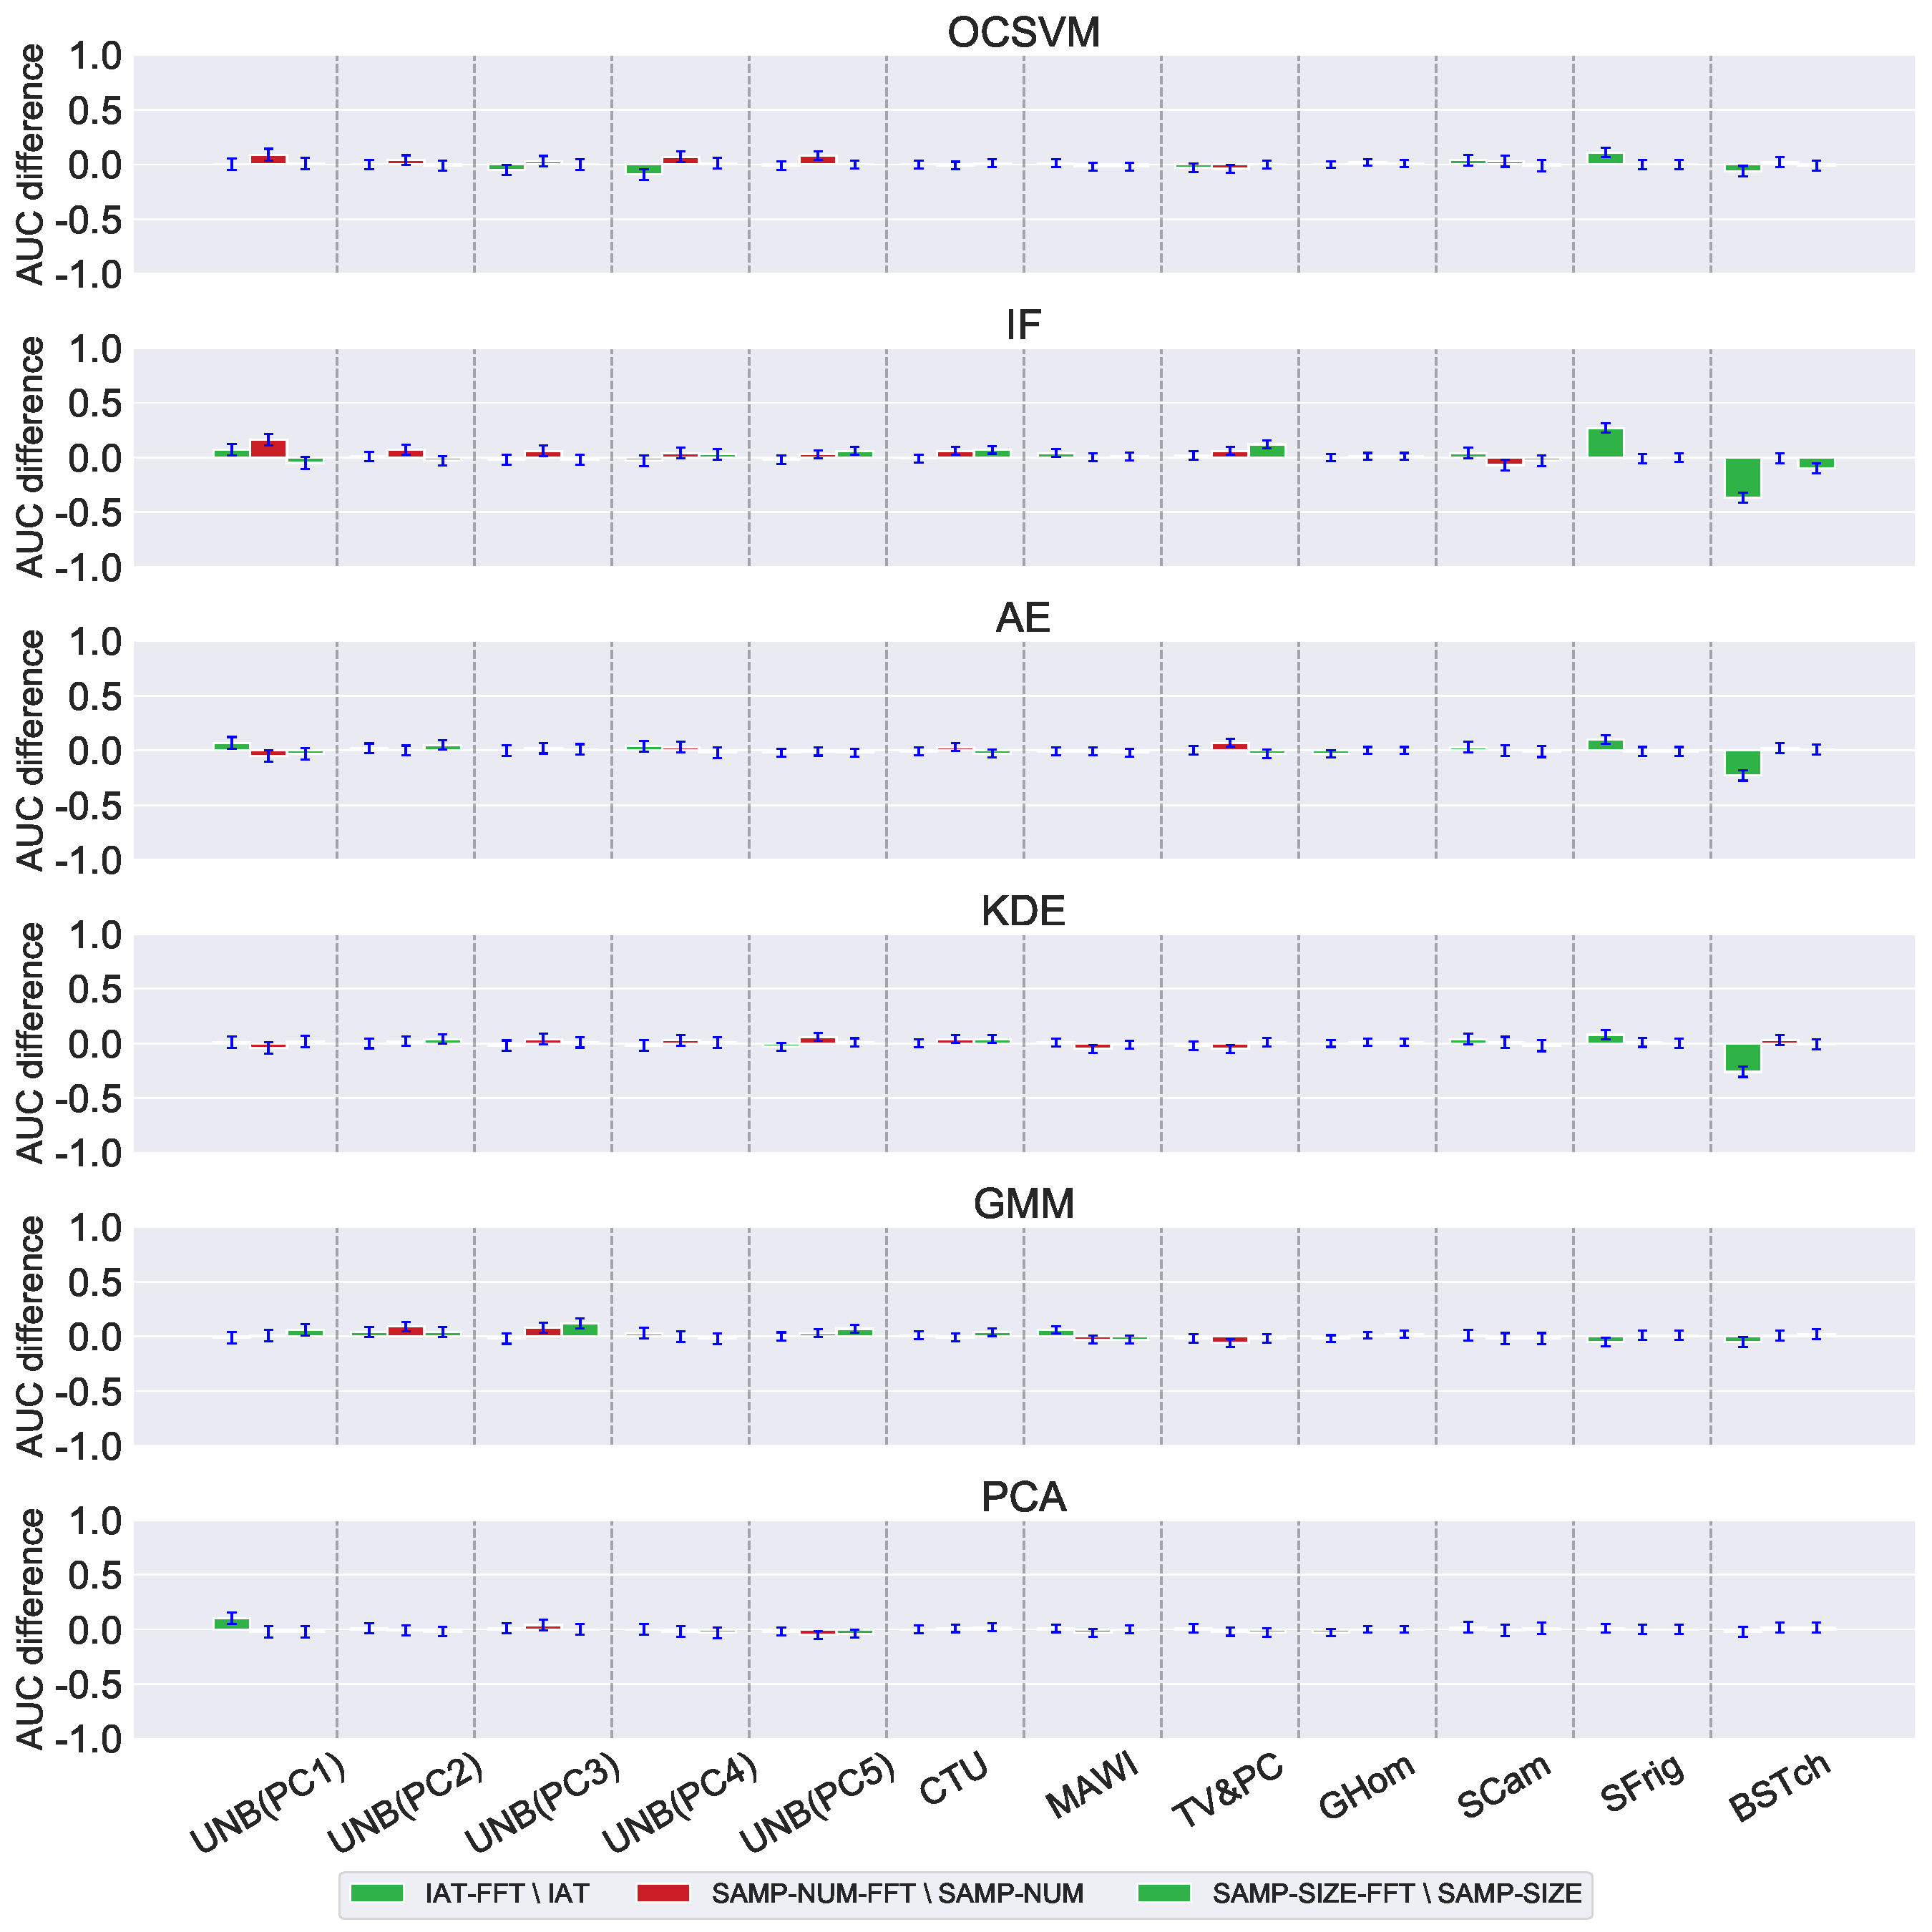
\includegraphics[width=0.99\textwidth, trim=0cm 0cm 0cm 0cm,clip]{OCSVM_IF_AE_KDE_GMM_PCA_with_best_parameters_on_basic_representations_diff.pdf}
\caption{The AUC difference}
\label{OCSVM_IF_AE_KDE_GMM_PCA_with_best_parameters_on_basic_representations_diff}
\end{figure}

% \vspace{12pt}
% \color{red}

\end{document}
